\section{Introduction}
Embedding images into generic features \old{is}\new{that can serve multiple purposes in computer vision has been} a long-standing problem.\old{in computer vision.} 
\new{First} \old{Initial} methods relied on handcrafted principles, such as SIFT~\citep{lowe2004distinctive}, before the scale of data and deep learning techniques allowed for end-to-end training. 
Pursuing generic feature embeddings is still relevant today, as collecting valuable annotated data for many \new{specific} tasks remains difficult.
This difficulty arises because of the required expertise (\emph{e.g.}, medical data, \new{or remote sensing}) or the cost at scale. 
Today, it is common to pretrain a model for a task for which plenty of data is available and extract a subset of the model to use as a feature extractor. 
Multiple approaches offer this possibility; supervised methods, building on classification or text-image alignment, allow training strong feature models to unlock downstream tasks. 
Alternatively, self-supervised methods building on the Transformer architecture have attracted significant attention due to \new{their high prediction performance on downstream tasks and the intriguing ability of some models to provide unsupervised segmentations~\citep{caron2021emerging}}\old{the emerging properties of the transforms they implement~\citep{caron2021emerging}.} 

In particular, the DINO algorithm is shown to produce models that contain explicit information about the semantic \old{segmentation}\new{layout} of an image.
Indeed, qualitative results show that the last attention layer naturally focuses on semantically consistent parts of \old{images.}\new{images and often produces interpretable attention maps.} 
Exploiting these properties, object discovery algorithms such as LOST \citep{simeoni2021localizing} build on top of DINO. 
Such algorithms can detect objects without supervision by gathering information in attention maps.
They are effectively unlocking a new frontier in computer vision. 

DINOv2~\citep{oquab2023dinov2}, a follow-up to DINO, provides features that allow tackling dense prediction tasks.
DINOv2 features \new{lead to successful}\old{strongly perform} monocular depth estimation and semantic segmentation with a frozen backbone and linear models.
Despite the strong performance on dense tasks, we observed that DINOv2 is surprisingly incompatible with LOST.
When used to extract features, it delivers disappointing performance, only on par with supervised alternative backbones in this scenario. 
\new{This suggests that DINOv2 behaves differently than DINO. The investigation described in this work notably exposes the presence of artefacts in the feature maps of DINOv2 that were not present in the first version of this model.}
\old{This suggests that a different behavior was introduced in the learning algorithm, and we set a goal to figure out what happened. 
The investigation described in this work exposes the presence of artifacts in the feature maps of DINOv2 that were not present in DINO.}
These are observable qualitatively using straightforward methods. 
\new{Also surprisingly}, applying the same observations to supervised \old{models}\new{vision transformers} exposes similar artifacts, as shown in Fig.~\ref{fig:allvits}.
This suggests that DINO is, in fact, an exception, while DINOv2 models match the baseline behavior of vision transformers. 

\begin{figure}[t]
  \centering
  {\footnotesize
  \setlength{\tabcolsep}{2.5pt} %
  \renewcommand{\arraystretch}{0.4} %
  \begin{tabular}{c cc cc cc }
    \vspace{0.2em}
    Input & DeiT-III-B & DeiT-III-L & OpenCLIP-B & OpenCLIP-L & DINO-B & DINOv2-g \\
    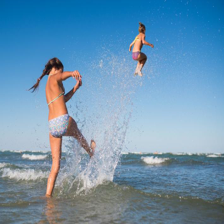
\includegraphics[width=0.13\textwidth]{resources/230914_1202_fig2_vizs_various_models/109_orig.png} &
    
\includegraphics[width=0.13\textwidth]{resources/230914_1202_fig2_vizs_various_models/deit3_base_patch16_224.fb_in22k_ft_in1k_109_lastattmap.png} &
    
\includegraphics[width=0.13\textwidth]{resources/230914_1202_fig2_vizs_various_models/deit3_large_patch16_224.fb_in22k_ft_in1k_109_lastattmap.png} &
    
\includegraphics[width=0.13\textwidth]{resources/230914_1202_fig2_vizs_various_models/vit_base_patch16_clip_224.laion2b_109_lastattmap.png} &
    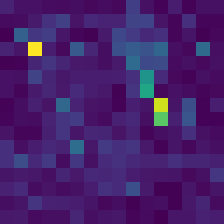
\includegraphics[width=0.13\textwidth]{resources/230914_1202_fig2_vizs_various_models/vit_large_patch14_clip_224.laion2b_109_lastattmap.png} &
    
\includegraphics[width=0.13\textwidth]{resources/230914_1202_fig2_vizs_various_models/vit_base_patch16_224.dino_109_lastattmap.png} &
    
\includegraphics[width=0.13\textwidth]{resources/230914_1202_fig2_vizs_various_models/vit_giant_patch14_dinov2.lvd142m_109_lastattmap.png}
    \\
    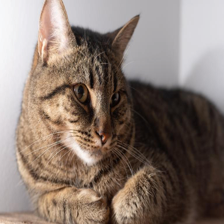
\includegraphics[width=0.13\textwidth]{resources/230914_1202_fig2_vizs_various_models/1500_orig.png} &
    
\includegraphics[width=0.13\textwidth]{resources/230914_1202_fig2_vizs_various_models/deit3_base_patch16_224.fb_in22k_ft_in1k_1500_lastattmap.png} &
    
\includegraphics[width=0.13\textwidth]{resources/230914_1202_fig2_vizs_various_models/deit3_large_patch16_224.fb_in22k_ft_in1k_1500_lastattmap.png} &
    
\includegraphics[width=0.13\textwidth]{resources/230914_1202_fig2_vizs_various_models/vit_base_patch16_clip_224.laion2b_1500_lastattmap.png} &
    
\includegraphics[width=0.13\textwidth]{resources/230914_1202_fig2_vizs_various_models/vit_large_patch14_clip_224.laion2b_1500_lastattmap.png} &
    
\includegraphics[width=0.13\textwidth]{resources/230914_1202_fig2_vizs_various_models/vit_base_patch16_224.dino_1500_lastattmap.png} &
    
\includegraphics[width=0.13\textwidth]{resources/230914_1202_fig2_vizs_various_models/vit_giant_patch14_dinov2.lvd142m_1500_lastattmap.png}
    \\
    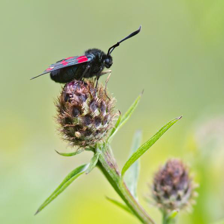
\includegraphics[width=0.13\textwidth]{resources/230914_1202_fig2_vizs_various_models/85_orig.png} &
    
\includegraphics[width=0.13\textwidth]{resources/230914_1202_fig2_vizs_various_models/deit3_base_patch16_224.fb_in22k_ft_in1k_85_lastattmap.png} &
    
\includegraphics[width=0.13\textwidth]{resources/230914_1202_fig2_vizs_various_models/deit3_large_patch16_224.fb_in22k_ft_in1k_85_lastattmap.png} &
    
\includegraphics[width=0.13\textwidth]{resources/230914_1202_fig2_vizs_various_models/vit_base_patch16_clip_224.laion2b_85_lastattmap.png} &
    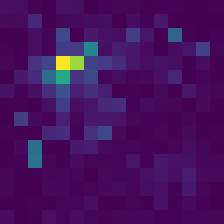
\includegraphics[width=0.13\textwidth]{resources/230914_1202_fig2_vizs_various_models/vit_large_patch14_clip_224.laion2b_85_lastattmap.png} &
    
\includegraphics[width=0.13\textwidth]{resources/230914_1202_fig2_vizs_various_models/vit_base_patch16_224.dino_85_lastattmap.png} &
    
\includegraphics[width=0.13\textwidth]{resources/230914_1202_fig2_vizs_various_models/vit_giant_patch14_dinov2.lvd142m_85_lastattmap.png}
    \\
    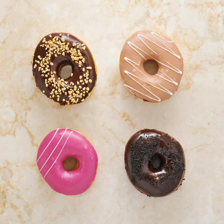
\includegraphics[width=0.13\textwidth]{resources/230914_1202_fig2_vizs_various_models/1753_orig.png} &
    
\includegraphics[width=0.13\textwidth]{resources/230914_1202_fig2_vizs_various_models/deit3_base_patch16_224.fb_in22k_ft_in1k_1753_lastattmap.png} &
    
\includegraphics[width=0.13\textwidth]{resources/230914_1202_fig2_vizs_various_models/deit3_large_patch16_224.fb_in22k_ft_in1k_1753_lastattmap.png} &
    
\includegraphics[width=0.13\textwidth]{resources/230914_1202_fig2_vizs_various_models/vit_base_patch16_clip_224.laion2b_1753_lastattmap.png} &
    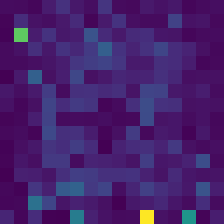
\includegraphics[width=0.13\textwidth]{resources/230914_1202_fig2_vizs_various_models/vit_large_patch14_clip_224.laion2b_1753_lastattmap.png} &
    
\includegraphics[width=0.13\textwidth]{resources/230914_1202_fig2_vizs_various_models/vit_base_patch16_224.dino_1753_lastattmap.png} &
    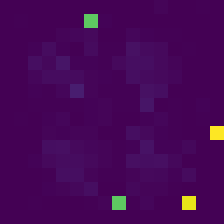
\includegraphics[width=0.13\textwidth]{resources/230914_1202_fig2_vizs_various_models/vit_giant_patch14_dinov2.lvd142m_1753_lastattmap.png}
    \\
  \end{tabular}
  }
  \caption{
    Illustration of artifacts observed in the attention maps of modern vision transformers. 
    We consider ViTs trained with label supervision (DeiT-III), text-supervision (OpenCLIP) or self-supervision (DINO and DINOv2).
    Interestingly, all models but DINO exhibit peaky outlier values in the attention maps.
    The goal of this work is to understand and mitigate this phenomenon.
  }  
  \label{fig:allvits}
\end{figure}

In this work, we set out to \new{better} understand this phenomenon \old{better} and develop methods to detect these artifacts.
We observe that they are tokens with \old{a}\new{roughly} 10x higher norm at the output and correspond to a small fraction of the total sequence (around 2\%).
We also show that these tokens appear around the middle layers of the vision transformer, and that they only appear after a sufficiently long training of a sufficiently big transformer.
In particular, we show that these outlier tokens appear in patches similar to their neighbors, meaning \new{patches that convey}\old{they bring} little additional information. \old{ to the vision transformer.}


\old{Additionally,} \new{As part of our investigation,} we evaluate the outlier tokens with simple linear models to \old{clarify}\new{understand} the information they contain.
We observe that, compared to non-outlier tokens, they hold less information about their original position in the image or the original pixels in their patch.
This observation suggests that the model discards the local information contained in these patches during inference. 
On the \old{contrary}\new{other hand}, learning an image classifier on outlier patches yields significantly stronger accuracy than doing so on the other patches, \new{suggesting that}
\old{This experiment indicates that} they contain global information about the image. 
We propose the following interpretation to these elements:
the model learns to recognize \old{tokens}\new{patches} containing little useful information, \old{discard this information by overwriting with higher-norm vectors,}and recycle \old{these}\new{the corresponding} tokens to aggregate global image information \new{while discarding spatial information}.

This interpretation is consistent with an inner mechanism in transformer models that allows performing computations within a restricted set of tokens. 
In order to test this hypothesis, we append additional tokens - that we call registers - to the token sequence, independent of the input image. 
We train several models with and without this modification and observe that the outlier tokens disappear from the sequence entirely. 
As a result, the performance of the models increases in dense prediction tasks, and the resulting feature maps are significantly smoother.
These smooth feature maps enable object discovery methods like LOST mentioned above with the updated models.

